\section{Optimizing of the Relaxation Factor}
\label{Sec: Optimizing Relaxation Factor}

As discussed in section \ref{Sub: Successive Over-Relaxation} is the successive over-relaxation (\acs{SOR}) method a well-known technique used to accelerate the convergence of the Gauss-Seidel algorithm. However, determining the optimal value of the relaxation factor $\omega$ is crucial, as it can vary based on the specifics of the problem and the geometry involved. The following section explores the optimization of the relaxation factor $\omega$ in the context of a three-dimensional flow of ionized particles around a charged sphere.

\begin{figure}[H]
    \centering
    \begin{subfigure}[b]{0.49\linewidth}
        \centering
        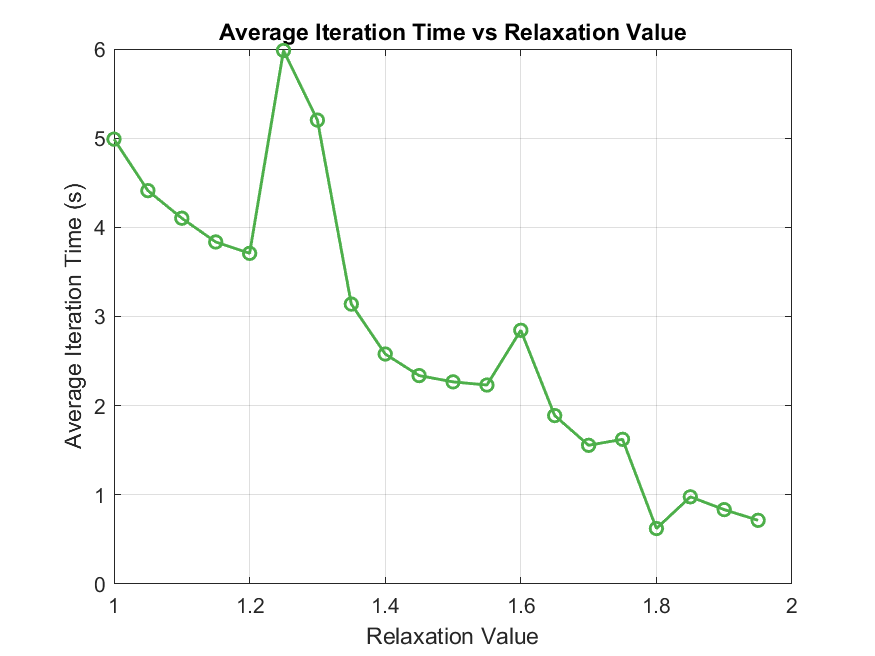
\includegraphics[width=\linewidth]{figures/overrelaxation/average_iteration_time_vs_relaxation_value.png}
        \caption{Average Iteration Time vs Relaxation Value}
        \label{fig:average_iteration_time}
    \end{subfigure}
    \hfill
    \begin{subfigure}[b]{0.49\linewidth}
        \centering
        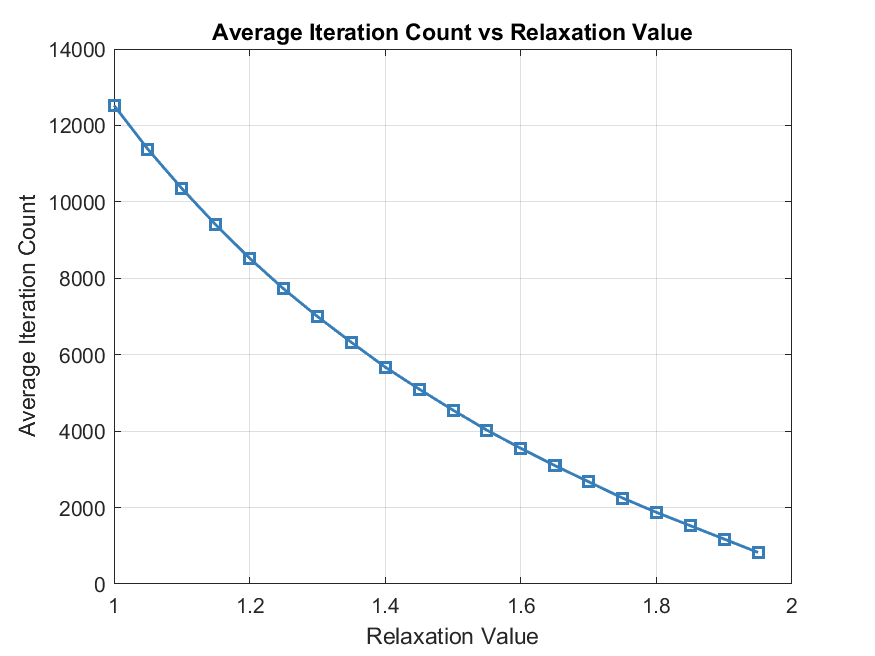
\includegraphics[width=\linewidth]{figures/overrelaxation/average_iteration_count_vs_relaxation_value.png}
        \caption{Average Iteration Count vs Relaxation Value}
        \label{fig:average_iteration_count}
    \end{subfigure}
    \caption{Comparison of Average Iteration Time and Count with Relaxation Values}
    \label{fig:comparison}
\end{figure}

The two figures suggest a clear improvement in convergence speed, both in terms of total computation time and iteration count, as the relaxation value $\omega$ approaches 2. Although the average iteration time fluctuates slightly, the overall trend shows a reduction in the time required per iteration for the \acs{GS}-algorithm. On the other hand, the iteration count follows a more stable and consistent trajectory, further indicating that a higher relaxation value leads to better performance. This finding contrasts with suggestions from the literature, where similar simulations recommend an optimal relaxation value of around 1.4 \cite{brieda_plasma_2019}. However, as previously mentioned, the optimal value for $\omega$ is highly dependent on the specific system configurations. Hence, the inclusion of an adaptive method for optimizing the relaxation factor could be a highly beneficial enhancement for improving convergence in future simulation setups \cite{brieda_plasma_2019}. Based on these results, the subsequent simulations presented in this report utilize a relaxation factor of 1.9 to optimize convergence efficiency.